\documentclass[]{article}
\usepackage{lmodern}
\usepackage{amssymb,amsmath}
\usepackage{ifxetex,ifluatex}
\usepackage{fixltx2e} % provides \textsubscript
\ifnum 0\ifxetex 1\fi\ifluatex 1\fi=0 % if pdftex
  \usepackage[T1]{fontenc}
  \usepackage[utf8]{inputenc}
\else % if luatex or xelatex
  \ifxetex
    \usepackage{mathspec}
    \usepackage{xltxtra,xunicode}
  \else
    \usepackage{fontspec}
  \fi
  \defaultfontfeatures{Mapping=tex-text,Scale=MatchLowercase}
  \newcommand{\euro}{€}
\fi
% use upquote if available, for straight quotes in verbatim environments
\IfFileExists{upquote.sty}{\usepackage{upquote}}{}
% use microtype if available
\IfFileExists{microtype.sty}{%
\usepackage{microtype}
\UseMicrotypeSet[protrusion]{basicmath} % disable protrusion for tt fonts
}{}
\usepackage[margin=1in]{geometry}
\usepackage{color}
\usepackage{fancyvrb}
\newcommand{\VerbBar}{|}
\newcommand{\VERB}{\Verb[commandchars=\\\{\}]}
\DefineVerbatimEnvironment{Highlighting}{Verbatim}{commandchars=\\\{\}}
% Add ',fontsize=\small' for more characters per line
\usepackage{framed}
\definecolor{shadecolor}{RGB}{248,248,248}
\newenvironment{Shaded}{\begin{snugshade}}{\end{snugshade}}
\newcommand{\KeywordTok}[1]{\textcolor[rgb]{0.13,0.29,0.53}{\textbf{{#1}}}}
\newcommand{\DataTypeTok}[1]{\textcolor[rgb]{0.13,0.29,0.53}{{#1}}}
\newcommand{\DecValTok}[1]{\textcolor[rgb]{0.00,0.00,0.81}{{#1}}}
\newcommand{\BaseNTok}[1]{\textcolor[rgb]{0.00,0.00,0.81}{{#1}}}
\newcommand{\FloatTok}[1]{\textcolor[rgb]{0.00,0.00,0.81}{{#1}}}
\newcommand{\CharTok}[1]{\textcolor[rgb]{0.31,0.60,0.02}{{#1}}}
\newcommand{\StringTok}[1]{\textcolor[rgb]{0.31,0.60,0.02}{{#1}}}
\newcommand{\CommentTok}[1]{\textcolor[rgb]{0.56,0.35,0.01}{\textit{{#1}}}}
\newcommand{\OtherTok}[1]{\textcolor[rgb]{0.56,0.35,0.01}{{#1}}}
\newcommand{\AlertTok}[1]{\textcolor[rgb]{0.94,0.16,0.16}{{#1}}}
\newcommand{\FunctionTok}[1]{\textcolor[rgb]{0.00,0.00,0.00}{{#1}}}
\newcommand{\RegionMarkerTok}[1]{{#1}}
\newcommand{\ErrorTok}[1]{\textbf{{#1}}}
\newcommand{\NormalTok}[1]{{#1}}
\usepackage{longtable,booktabs}
\usepackage{graphicx}
\makeatletter
\def\maxwidth{\ifdim\Gin@nat@width>\linewidth\linewidth\else\Gin@nat@width\fi}
\def\maxheight{\ifdim\Gin@nat@height>\textheight\textheight\else\Gin@nat@height\fi}
\makeatother
% Scale images if necessary, so that they will not overflow the page
% margins by default, and it is still possible to overwrite the defaults
% using explicit options in \includegraphics[width, height, ...]{}
\setkeys{Gin}{width=\maxwidth,height=\maxheight,keepaspectratio}
\ifxetex
  \usepackage[setpagesize=false, % page size defined by xetex
              unicode=false, % unicode breaks when used with xetex
              xetex]{hyperref}
\else
  \usepackage[unicode=true]{hyperref}
\fi
\hypersetup{breaklinks=true,
            bookmarks=true,
            pdfauthor={Lars Vilhuber},
            pdftitle={Snapshot S2014 availability},
            colorlinks=true,
            citecolor=blue,
            urlcolor=blue,
            linkcolor=magenta,
            pdfborder={0 0 0}}
\urlstyle{same}  % don't use monospace font for urls
\setlength{\parindent}{0pt}
\setlength{\parskip}{6pt plus 2pt minus 1pt}
\setlength{\emergencystretch}{3em}  % prevent overfull lines
\setcounter{secnumdepth}{0}

%%% Use protect on footnotes to avoid problems with footnotes in titles
\let\rmarkdownfootnote\footnote%
\def\footnote{\protect\rmarkdownfootnote}

%%% Change title format to be more compact
\usepackage{titling}

% Create subtitle command for use in maketitle
\newcommand{\subtitle}[1]{
  \posttitle{
    \begin{center}\large#1\end{center}
    }
}

\setlength{\droptitle}{-2em}
  \title{Snapshot S2014 availability}
  \pretitle{\vspace{\droptitle}\centering\huge}
  \posttitle{\par}
  \author{Lars Vilhuber}
  \preauthor{\centering\large\emph}
  \postauthor{\par}
  \date{}
  \predate{}\postdate{}



\begin{document}

\maketitle


There are as of this date two versions of the MOU that binds the Census
Bureau and state agencies in effect: The original MOU, signed when the
state first joined the LED Program, and a successor MOU, mostly
standardized across states, that states signed when the first MOU
expired after 10 years. The original MOU affected research access to the
S2008 snapshot. Access to subsequent snapshots has been contingent on a
mixture of both.

\begin{Shaded}
\begin{Highlighting}[]
\CommentTok{# version of MOU we are interested in}
\NormalTok{mouversion <-}\StringTok{ }\DecValTok{2}
\NormalTok{mouoption    <-}\StringTok{ "A"} 
\CommentTok{# this could also be "http://download.vrdc.cornell.edu/qwipu/"}
\NormalTok{urlbase <-}\StringTok{ "http://lehd.ces.census.gov/pub/"}
\CommentTok{# this could also be "latest_release"}
\CommentTok{# qwivintage <- "R2015Q3"}
\NormalTok{qwivintage <-}\StringTok{ "latest_release"}
\NormalTok{qwistates <-}\StringTok{ "AK AL AR AZ CA CO CT DC DE FL GA HI IA ID IL IN KS KY LA MA MD ME MI MN MO MS MT NC ND NE NH NJ NM NV NY OH OK OR PA RI SC SD TN TX UT VA VT WA WI WV WY"}
\NormalTok{qwistates <-}\StringTok{ }\KeywordTok{unlist}\NormalTok{(}\KeywordTok{strsplit}\NormalTok{(qwistates,}\StringTok{" "}\NormalTok{))}
\CommentTok{# common quarter to look at}
\CommentTok{# this could be deduced from metadata, here we hard-code it}
\NormalTok{qwiyear    <-}\StringTok{ }\DecValTok{2014}
\NormalTok{qwiquarter <-}\StringTok{ }\DecValTok{1}
\end{Highlighting}
\end{Shaded}

We obtained a list of the state of the MOUs as of 12-10-2015. From it,
we will use the later versions (version 2) that have selected ``Option
A'', as those are the ones that have delegated granting access to the
Census Bureau's review process. The other options are not an ex-ante
``No'', but currently, no data is available to assess whether a research
project will be approved by the individual states.

\begin{longtable}[c]{@{}rllrll@{}}
\toprule
fips & Abbr & Name & Version & Option & OldOption\tabularnewline
\midrule
\endhead
1 & AL & Alabama & 2 & B &\tabularnewline
2 & AK & Alaska & 1 & NA & B\tabularnewline
4 & AZ & Arizona & 2 & A &\tabularnewline
5 & AR & Arkansas & 2 & A &\tabularnewline
6 & CA & California & 2 & B &\tabularnewline
8 & CO & Colorado & 2 & B &\tabularnewline
9 & CT & Connecticut & 2 & B &\tabularnewline
10 & DE & Delaware & 2 & A &\tabularnewline
11 & DC & District of Columbia & 2 & A &\tabularnewline
12 & FL & Florida & 2 & B &\tabularnewline
13 & GA & Georgia & 2 & B &\tabularnewline
66 & GU & Guam & NA & NA & NA\tabularnewline
15 & Hi & Hawaii & 3 & B &\tabularnewline
16 & ID & Idaho & 2 & B &\tabularnewline
17 & IL & Illinois & 1 & A &\tabularnewline
18 & IN & Indiana & 2 & A &\tabularnewline
19 & IA & Iowa & 2 & A &\tabularnewline
20 & KS & Kansas & 2 & A &\tabularnewline
21 & KY & Kentucky & 2 & B &\tabularnewline
22 & LA & Louisiana & 1 & A &\tabularnewline
23 & ME & Maine & 2 & A &\tabularnewline
24 & MD & Maryland & 1 & A &\tabularnewline
25 & MA & Massachusetts & 2 & B &\tabularnewline
26 & MI & Michigan & 1 & NA & B\tabularnewline
27 & MN & Minnesota & 2 & B &\tabularnewline
28 & MS & Mississippi & 1 & NA & B\tabularnewline
29 & MO & Missouri & 2 & B &\tabularnewline
30 & MT & Montana & 2 & B &\tabularnewline
31 & NE & Nebraska & 1 & NA & B\tabularnewline
32 & NV & Nevada & 2 & A &\tabularnewline
33 & NH & New Hampshire & 2 & B &\tabularnewline
34 & NJ & New Jersey & 2 & B &\tabularnewline
35 & NM & New Mexico & 2 & B &\tabularnewline
36 & NY & New York & 1 & NA & B\tabularnewline
37 & NC & North Carolina & 2 & B &\tabularnewline
38 & ND & North Dakota & 2 & B &\tabularnewline
39 & OH & Ohio & 1 & NA & B\tabularnewline
40 & OK & Oklahoma & 2 & A &\tabularnewline
41 & OR & Oregon & 2 & B &\tabularnewline
42 & PA & Pennsylvania & 2 & B &\tabularnewline
72 & PR & Puerto Rico & 1 & NA & NA\tabularnewline
44 & RI & Rhode Island & 2 & B &\tabularnewline
45 & SC & South Carolina & 2 & B &\tabularnewline
46 & SD & South Dakota & 1 & NA & B\tabularnewline
47 & TN & Tennessee & 2 & A &\tabularnewline
48 & TX & Texas & 2 & B &\tabularnewline
49 & UT & Utah & 2 & B &\tabularnewline
50 & VT & Vermont & 2 & B &\tabularnewline
78 & VI & Virgin Islands & 1 & NA & NA\tabularnewline
51 & VA & Virginia & 2 & B &\tabularnewline
53 & WA & Washington & 2 & B &\tabularnewline
54 & WV & West Virginia & 2 & B &\tabularnewline
55 & WI & Wisconsin & 2 & B &\tabularnewline
56 & WY & Wyoming & 1 & NA & B\tabularnewline
\bottomrule
\end{longtable}

We first define (source) a function to download QWI CSV files.

\begin{Shaded}
\begin{Highlighting}[]
\KeywordTok{source}\NormalTok{(}\StringTok{"download_qwi.R"}\NormalTok{,}\DataTypeTok{echo =} \OtherTok{TRUE}\NormalTok{)}
\end{Highlighting}
\end{Shaded}

\begin{verbatim}
## 
## > download_qwi <- function(state) {
## +     qwifile <- paste("qwi", tolower(state), "sa_f_gs_ns_oslp_u", 
## +         sep = "_")
## +     con <- gzcon(url(pa .... [TRUNCATED]
\end{verbatim}

We then cycle through all the states and download the relevant file.

\begin{Shaded}
\begin{Highlighting}[]
\NormalTok{time.qwi <-}\StringTok{ }\KeywordTok{system.time}\NormalTok{(for (x in qwistates) \{ }
  \KeywordTok{eval}\NormalTok{(}\KeywordTok{parse}\NormalTok{(}\DataTypeTok{text=}\KeywordTok{paste}\NormalTok{(}\StringTok{"qwi_"}\NormalTok{,}\KeywordTok{tolower}\NormalTok{(x),}\StringTok{" <- download_qwi(}\CharTok{\textbackslash{}"}\StringTok{"}\NormalTok{,x,}\StringTok{"}\CharTok{\textbackslash{}"}\StringTok{)"}\NormalTok{,}\DataTypeTok{sep =} \StringTok{""}\NormalTok{)))}
  \NormalTok{\})}
\end{Highlighting}
\end{Shaded}

The above code can take a while. The above code ran for 24 minutes.

Now that we have the files, we collate them all into a single file:

\begin{Shaded}
\begin{Highlighting}[]
\NormalTok{for (x in qwistates) \{ }\KeywordTok{eval}\NormalTok{(}\KeywordTok{parse}\NormalTok{(}\DataTypeTok{text=}\KeywordTok{paste}\NormalTok{(}\StringTok{"qwi_"}\NormalTok{,}\KeywordTok{tolower}\NormalTok{(x),}\StringTok{"$state = }\CharTok{\textbackslash{}"}\StringTok{"}\NormalTok{,x,}\StringTok{"}\CharTok{\textbackslash{}"}\StringTok{"}\NormalTok{,}\DataTypeTok{sep =} \StringTok{""}\NormalTok{)))\}}
\NormalTok{for (x in qwistates[}\DecValTok{1}\NormalTok{]) \{ }\KeywordTok{eval}\NormalTok{(}\KeywordTok{parse}\NormalTok{(}\DataTypeTok{text=}\KeywordTok{paste}\NormalTok{(}\StringTok{"all <- qwi_"}\NormalTok{,}\KeywordTok{tolower}\NormalTok{(x),}\DataTypeTok{sep =} \StringTok{""}\NormalTok{)))\}}
\NormalTok{for (x in qwistates[-}\DecValTok{1}\NormalTok{]) \{ }\KeywordTok{eval}\NormalTok{(}\KeywordTok{parse}\NormalTok{(}\DataTypeTok{text=}\KeywordTok{paste}\NormalTok{(}\StringTok{"all <- rbind(all,qwi_"}\NormalTok{,}\KeywordTok{tolower}\NormalTok{(x),}\StringTok{")"}\NormalTok{,}\DataTypeTok{sep =} \StringTok{""}\NormalTok{)))\}}
\end{Highlighting}
\end{Shaded}

and merge on the indicators for MOU status:

\begin{Shaded}
\begin{Highlighting}[]
\NormalTok{allmous <-}\StringTok{ }\KeywordTok{merge}\NormalTok{(all,mous,}\DataTypeTok{by.x=}\StringTok{"geography"}\NormalTok{,}\DataTypeTok{by.y =} \StringTok{"fips"}\NormalTok{,}\DataTypeTok{all.x =} \OtherTok{TRUE}\NormalTok{)}
\NormalTok{size <-}\StringTok{ }\NormalTok{allmous[allmous$ind_level==}\StringTok{"A"}\NormalTok{,]}
\NormalTok{industry <-}\StringTok{ }\NormalTok{allmous[allmous$industry !=}\StringTok{ "00"}\NormalTok{,]}
\end{Highlighting}
\end{Shaded}

The industry distribution of \textbf{Emp} by chosen option thus looks
like this:
\begin{figure}
\centering
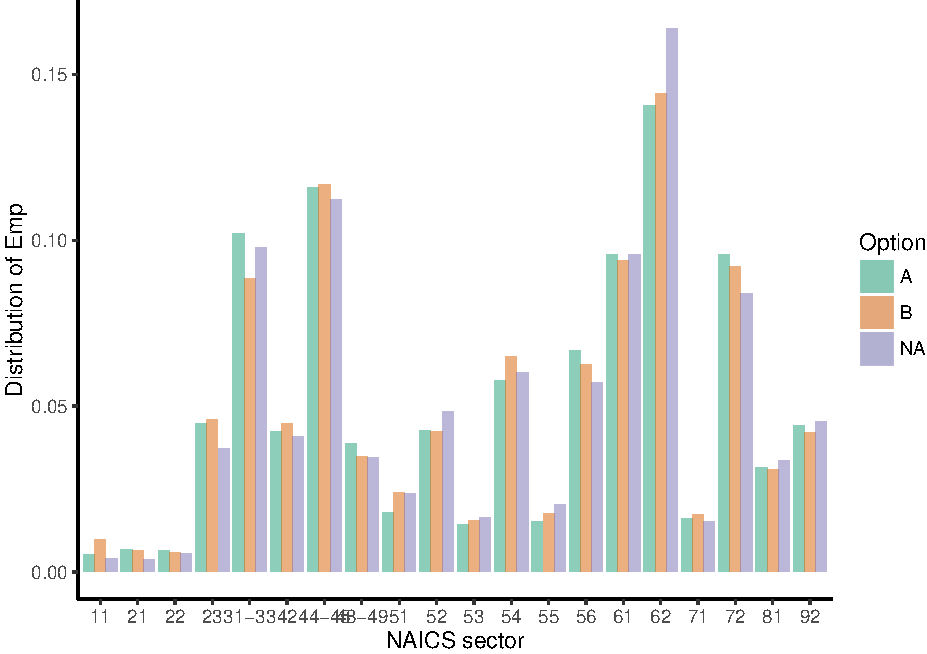
\includegraphics[width=0.8\textwidth]{s2014_availability_files/figure-latex/graph_Emp-1.pdf}
\end{figure}

For the industry distribution of \textbf{SepBeg}, the distribution looks
like this:
\begin{figure}
\centering
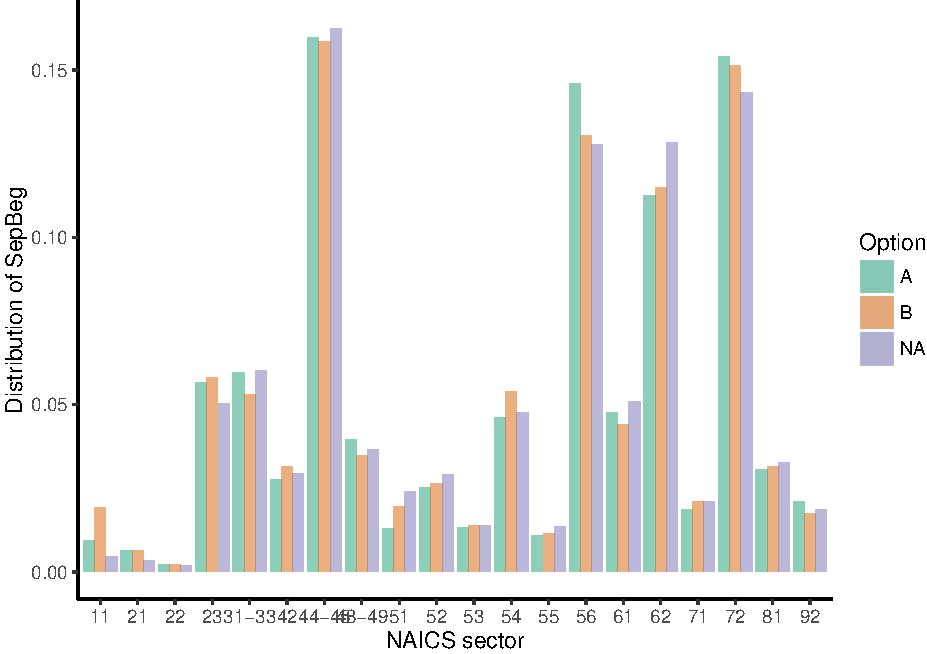
\includegraphics[width=0.8\textwidth]{s2014_availability_files/figure-latex/graph_SepBeg-1.pdf}
\end{figure}

For the industry distribution of \textbf{Payroll}, the distribution
looks like this:
\begin{figure}
\centering
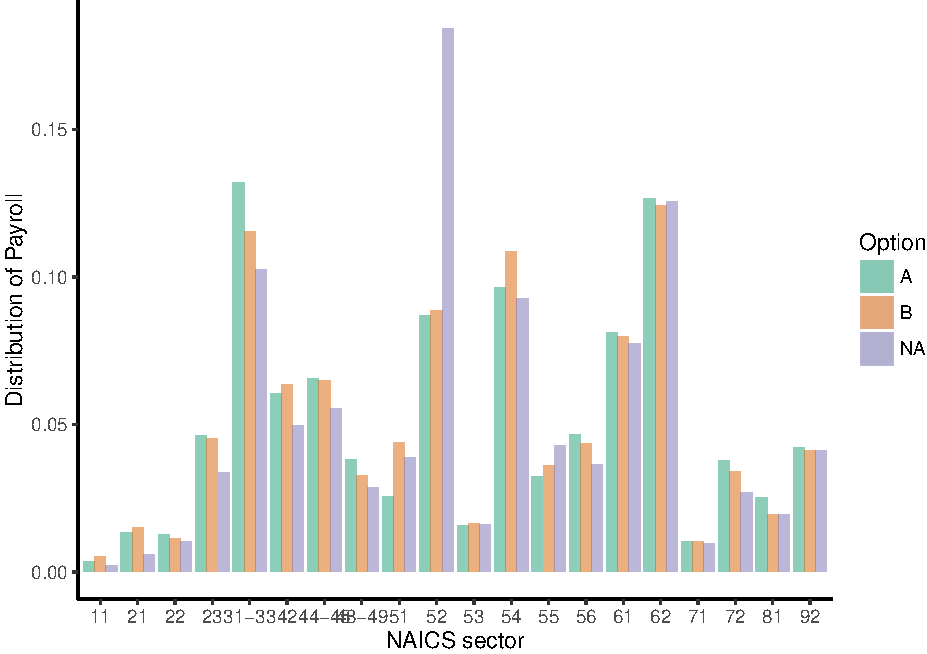
\includegraphics[width=0.8\textwidth]{s2014_availability_files/figure-latex/graph_Payroll-1.pdf}
\end{figure}

Additional variables (see the
\href{LEHD\%20Schema}{\url{http://lehd.ces.census.gov/data/schema/V4.0.4/lehd_public_use_schema.html}}
for names) can be easily added to the Rmd source file.

\end{document}
